\documentclass{article}

\usepackage{hyperref}
\hypersetup{
	colorlinks=true,
	linkcolor=blue,
	filecolor=magenta,
	urlcolor=cyan,
}
\usepackage{graphicx}
\graphicspath{ {./screenshots/} }

\title{Testing Policy Document}
\author{devs101}


\begin{document}

\maketitle
\newpage
\section{Testing Process}
Unit testing is done on each individual module of the application, and end-to-end integration
testing is done to ensure that the UI works as expected and integrates all the modules in the 
required fashion. Unit testing is done during development of a feature by the developer(s) working
on that feature. When that feature is done and merged into the main development branch, the
integration tests are run to ensure that the feature has not altered the correctness of the
application as a whole. Automated testing is also performed on Travis CI. Any pushes to
the development or master branch automatically runs both unit and integration tests, and
reports the result on the GitHub repo. The developers also run the Google Lighthouse
auditing system to ensure that the website meets modern webapp standards. The unit and
integration testing covers the functional requirements of the system, and the Lighthouse audit
ensures adherence to non-functional requirements such as accessibility and performance.

\section{Testing Tools}
For unit testing, the Jest framework for Node.js is used. Jest is installed as a Node
module. The Jest configuration is stored as a part of the code, so new developers need not
configure the module. In order to create a new test suite, the developer should create a
new JavaScript file in the folder test/unit/specs. The filename should have the format
"name.spec.js". It is imperative that the filename includes the "spec" portion, as that is
what Jest uses to separate normal source code files from spec files.
Jest tests are written using three main methods: describe(), it(), and expect().
The tester uses the describe() method to group a series of tests to a particular module.
The tester then asserts what the module should or should not do, using the it() function.
An example usage would be it('throws an appropriate error when x occurs', test), where
test is a function that performs a series of assertions with the expect() function.
A trivial example of a passing assertion would be expect(true).toEqual(true). The tests
are executed asynchronously, so the tester should ensure that tests do not depend on the
outcome of other tests, as that would lead to a race condition. For more detailed
descriptions of how to write tests, the developer is referred to the 
\href{https://jestjs.io/docs/en/using-matchers}{Jest Documentation}.

For integration testing, the Cypress end-to-end testing framework for Node.js is used.
Similar to the unit testing, the cypress module is already configured. In order to
create a new test suite, the developer should create a file with the format "name.spec.js"
under the folder test/integration/specs. Again, the spec part of the filename is important,
as Cypress uses that to determine test suites. The Cypress tests are written in a similar fashion
to the Jest tests, also using the describe() and it() functions in the same fashion. However,
Cypress tests use different functions to visit webpages, and perform actions on elements.
The basic commands are cy.visit('<url>'), which will visit the webpage, and pass if it
loads correctly, and cy.get('selector'), where the selector is any valid html selector,
including '.classname', and '\#id'. This will pass if the element exists and is visible.
The should() method performs some kind of assertion on the element. Elements can also be interacted
with via methods such as click() and type('text').
Commands can be chained together to perform complex assertions, for example,
cy.get('\#textbox').click().type('Hello').should('be.visible').should('have.value', 'Hello').
This chain will get the element with the ID of 'textbox', and then click on it, and type
'Hello' into it, and then assert that it is visible, and that it has a value of 'Hello'.
For more in depth instructions on how to use Cypress, the developer is referred to 
\href{https://docs.cypress.io/api/introduction/api.html#Sections}{Cypress Documentation}.

\section{Test Cases}
The unit test cases are stored at\\
\href{https://github.com/dolan212/devs101/tree/master/test/unit/specs}{https://github.com/dolan212/devs101/tree/master/test/unit/specs}.\\
Unit tests are executed using the "test" npm script. Assuming the developer has npm installed,
they can run "npm run test" to execute the unit tests. Jest will automatically
detect the spec files, and run the tests, producing a report at the end, as well as
realtime feedback. \\
The integration test cases are stored at\\
\href{https://github.com/dolan212/devs101/tree/master/test/integration/specs}{https://github.com/dolan212/devs101/tree/master/test/integration/specs}.\\
Integration tests are run using the "cy:open" npm script. The integration tests require
that the development server be running already. To run the development server, run
"npm run dev". Then, in another terminal, run "npm run cy:open". This will open
the Cypress testing window, which will display a list of all the spec files.
Select a test file to run all tests in that file. If the developer has Google Chrome,
or any Chrome based browser, the tests will be run in that browser, otherwise
Cypress' built in Electron based browser will be used. The developer can watch
in real time as the tests are performed, and the webpage is interacted with.
For automated testing, the integration-test npm script is used, however, this
requires the Cypress recording key to be saved as an environment variable, in order
to record the test cases and upload them to the Cypress dashboard, hence it is only
applicable to automated testing, and is not intended for use by the developer directly.

\newpage
\section{History}
The history of test builds can be found \href{https://travis-ci.org/dolan212/devs101/builds}{Here},
with saved logs of each build. Our Cypress runs can be found \href{https://dashboard.cypress.io/#/projects/v87qtg/runs}{Here}.\\
\subsection{Screenshots}
\begin{figure}[h]
    \centering
    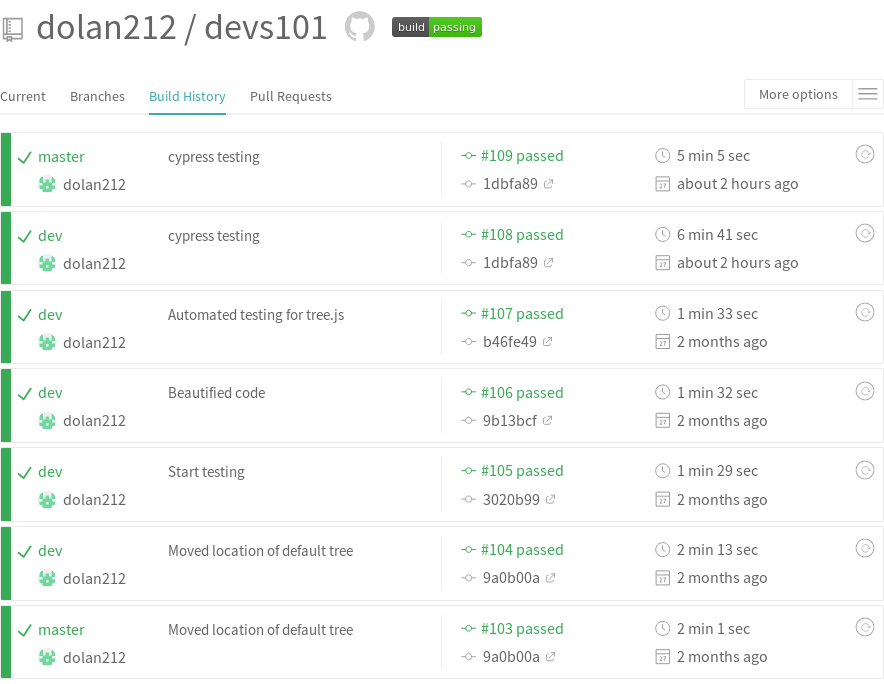
\includegraphics[width=\textwidth]{travis_history}
    \caption{most recent history of Travis builds}
\end{figure}

\begin{figure}[h]
    \centering
    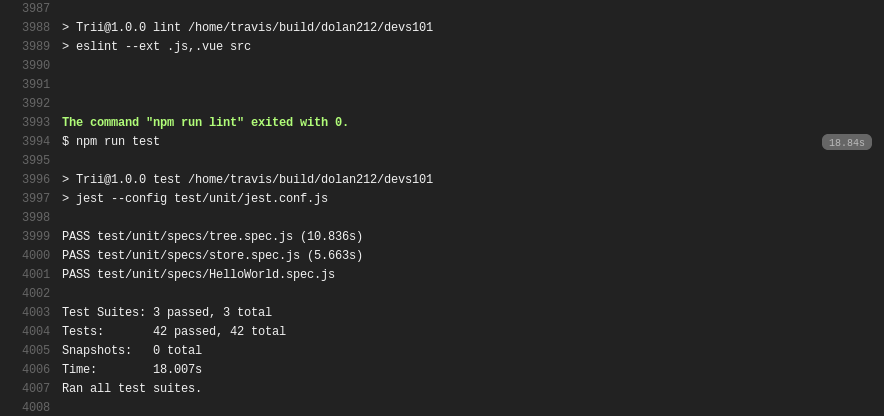
\includegraphics[width=\textwidth]{travis_run_1}
    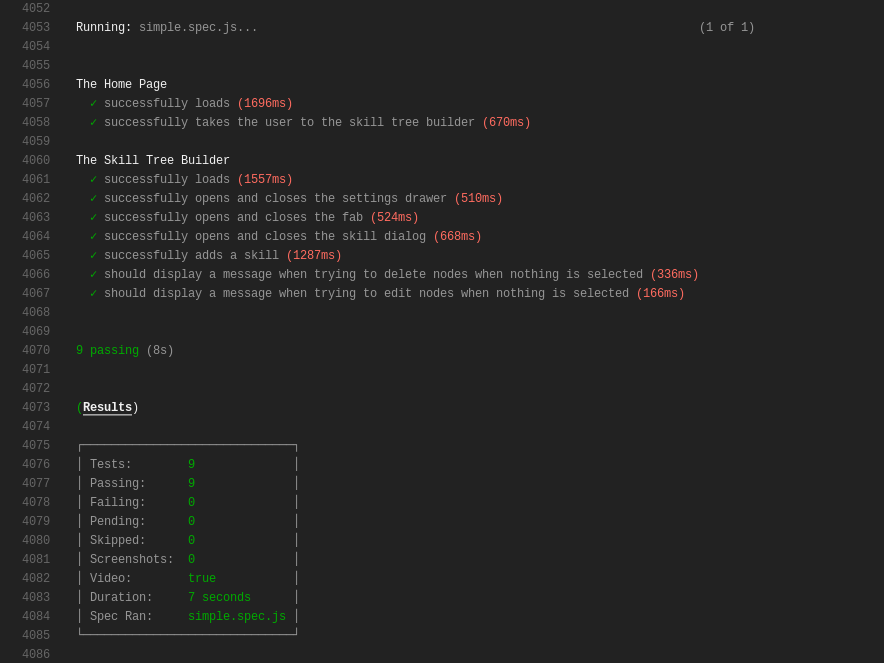
\includegraphics[width=\textwidth]{travis_run_2}
    \caption{test output on recent Travis build}
\end{figure}

\begin{figure}[h]
    \centering
    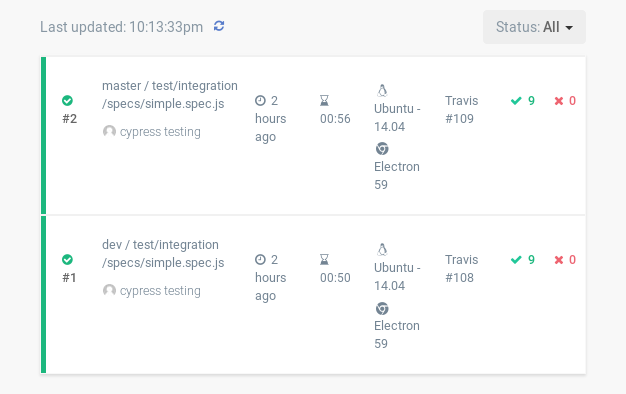
\includegraphics[width=\textwidth]{cypress_dashboard}
    \caption{Cypress dashboard}
\end{figure}

\begin{figure}[h]
    \centering
    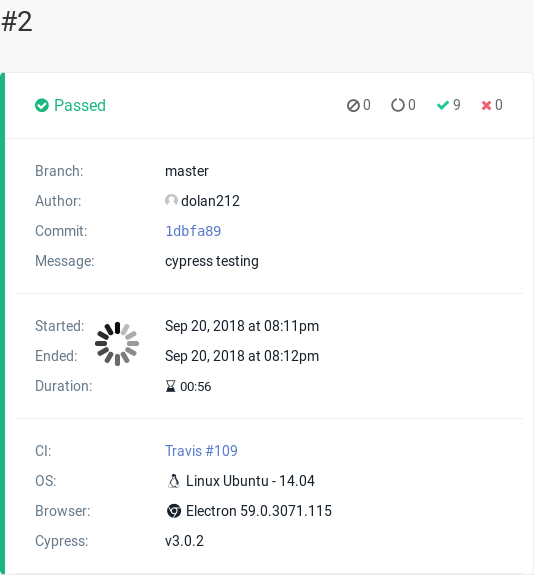
\includegraphics[width=\textwidth]{cypress_run_1}
    \caption{details of a Cypress run}
\end{figure}
\begin{figure}[h]
    \centering
    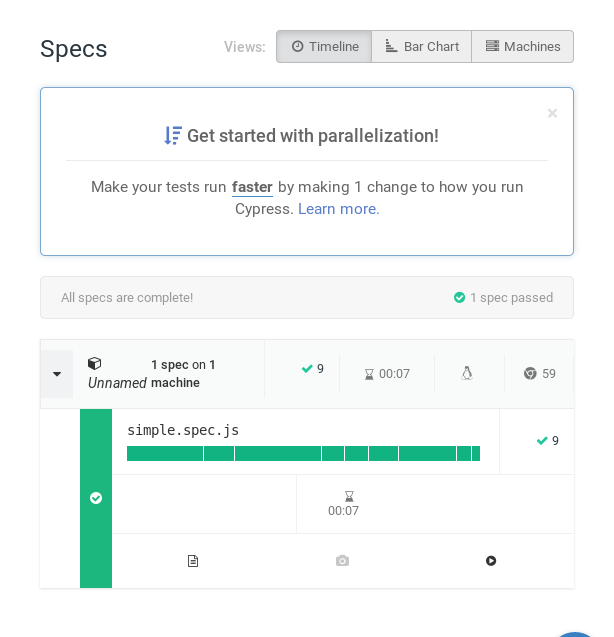
\includegraphics[width=\textwidth]{cypress_run_2}
    \caption{details of specs for a Cypress run}
\end{figure}

\end{document}
